\documentclass[tikz,border=10pt]{standalone}
\usepackage{pgfplots}
\pgfplotsset{compat=newest}
% \pgfplotsset{compat=1.18}
\usepackage[american]{circuitikz}
\usepackage{cmbright}
\usetikzlibrary{fit}

\definecolor{myred}{RGB}{170,0,0}
\definecolor{myblue}{RGB}{0,0,220}
\definecolor{mygreen}{RGB}{0,150,0}
\definecolor{myorange}{RGB}{255,127,0}
\definecolor{mybrown}{RGB}{150,75,0}

\ctikzset{bipoles/resistor/height=0.2}
\ctikzset{bipoles/resistor/width=0.5}
\ctikzset{bipoles/capacitor/height=0.4}
\ctikzset{bipoles/capacitor/width=0.15}


\begin{document}
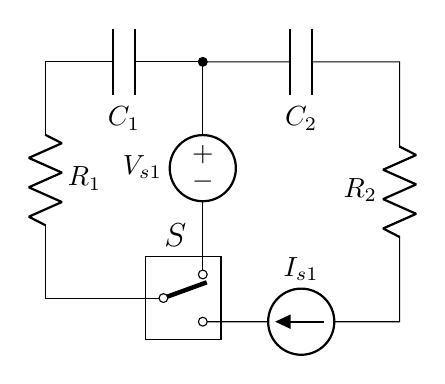
\begin{tikzpicture}
\begin{scope}
    % Define nodes
    \draw (0, 0) node[circ] (A1) {};
    \draw (0, -2.7) node[ocirc] (B1) {};
    \draw (0, -3.3) node[ocirc] (B2) {};
    \draw (-0.5, -3) node[ocirc] (B0) {};

    % Left loop: Voltage source and resistors
    \draw (-2, -3)
        to[R, l_={$R_1$}] ++(0, 3)
        to[C, l_={$C_1$}] (A1)
        to[V, l_={$V_{s1}$}] (B1);
    \draw (-2, -3) to (B0);
    \node at ($(B0) + (0.15, 0.8)$) {\large $S$};

    % Cap between A1 and B1
    \draw (A1)
        to[C, l_={$C_2$}] ++(2.5, 0)
        to[R, l_={$R_2$}] ++(0, -3.3)
        to[I, l_={$I_{s1}$}] (B2);
    
        % Draw switch arm
    \draw[ultra thick] (B0) to ($(B1) + (0.05, -0.10)$);

    % Box around the switch
    \node[draw=black, thin, fit=(B0) (B1) (B2), inner sep=5pt] {};
\end{scope}
\end{tikzpicture}

\end{document}